% Options for packages loaded elsewhere
\PassOptionsToPackage{unicode}{hyperref}
\PassOptionsToPackage{hyphens}{url}
%
\documentclass[
  a4paper,
]{scrbook}

\usepackage{amsmath,amssymb}
\usepackage{iftex}
\ifPDFTeX
  \usepackage[T1]{fontenc}
  \usepackage[utf8]{inputenc}
  \usepackage{textcomp} % provide euro and other symbols
\else % if luatex or xetex
  \usepackage{unicode-math}
  \defaultfontfeatures{Scale=MatchLowercase}
  \defaultfontfeatures[\rmfamily]{Ligatures=TeX,Scale=1}
\fi
\usepackage{lmodern}
\ifPDFTeX\else  
    % xetex/luatex font selection
  \setmainfont[]{Latin Modern Roman}
  \setsansfont[]{Latin Modern Roman}
\fi
% Use upquote if available, for straight quotes in verbatim environments
\IfFileExists{upquote.sty}{\usepackage{upquote}}{}
\IfFileExists{microtype.sty}{% use microtype if available
  \usepackage[]{microtype}
  \UseMicrotypeSet[protrusion]{basicmath} % disable protrusion for tt fonts
}{}
\makeatletter
\@ifundefined{KOMAClassName}{% if non-KOMA class
  \IfFileExists{parskip.sty}{%
    \usepackage{parskip}
  }{% else
    \setlength{\parindent}{0pt}
    \setlength{\parskip}{6pt plus 2pt minus 1pt}}
}{% if KOMA class
  \KOMAoptions{parskip=half}}
\makeatother
\usepackage{xcolor}
\setlength{\emergencystretch}{3em} % prevent overfull lines
\setcounter{secnumdepth}{5}
% Make \paragraph and \subparagraph free-standing
\ifx\paragraph\undefined\else
  \let\oldparagraph\paragraph
  \renewcommand{\paragraph}[1]{\oldparagraph{#1}\mbox{}}
\fi
\ifx\subparagraph\undefined\else
  \let\oldsubparagraph\subparagraph
  \renewcommand{\subparagraph}[1]{\oldsubparagraph{#1}\mbox{}}
\fi


\providecommand{\tightlist}{%
  \setlength{\itemsep}{0pt}\setlength{\parskip}{0pt}}\usepackage{longtable,booktabs,array}
\usepackage{calc} % for calculating minipage widths
% Correct order of tables after \paragraph or \subparagraph
\usepackage{etoolbox}
\makeatletter
\patchcmd\longtable{\par}{\if@noskipsec\mbox{}\fi\par}{}{}
\makeatother
% Allow footnotes in longtable head/foot
\IfFileExists{footnotehyper.sty}{\usepackage{footnotehyper}}{\usepackage{footnote}}
\makesavenoteenv{longtable}
\usepackage{graphicx}
\makeatletter
\def\maxwidth{\ifdim\Gin@nat@width>\linewidth\linewidth\else\Gin@nat@width\fi}
\def\maxheight{\ifdim\Gin@nat@height>\textheight\textheight\else\Gin@nat@height\fi}
\makeatother
% Scale images if necessary, so that they will not overflow the page
% margins by default, and it is still possible to overwrite the defaults
% using explicit options in \includegraphics[width, height, ...]{}
\setkeys{Gin}{width=\maxwidth,height=\maxheight,keepaspectratio}
% Set default figure placement to htbp
\makeatletter
\def\fps@figure{htbp}
\makeatother

\usepackage{booktabs}
\usepackage{longtable}
\usepackage{array}
\usepackage{multirow}
\usepackage{wrapfig}
\usepackage{float}
\usepackage{colortbl}
\usepackage{pdflscape}
\usepackage{tabu}
\usepackage{threeparttable}
\usepackage{threeparttablex}
\usepackage[normalem]{ulem}
\usepackage{makecell}
\usepackage{xcolor}
\usepackage{titling}
\setlength{\droptitle}{-2cm}
\preauthor{
  \begin{center}
  \Large
  \vspace{10mm}
  by

  \vspace{20mm}
}
\postauthor{
  \end{center}
  \vfill
}

\predate{
  \begin{center}
  A thesis 
  submitted in fulfilment of the \\
  requirements of the degree of \\
  Doctor of Philosophy in Physics\\               % Degree
  School of Physical and Chemical Sciences\\          % Department
  Te Herenga Waka - Victoria University of Wellington\\                       % University 
  \vspace{5mm}
}
\postdate{
  \\
  
\includegraphics[width=3in,height=1.5in]{figures/VUW-logo.png}\\
  \end{center}
  }
\makeatletter
\makeatother
\makeatletter
\@ifpackageloaded{bookmark}{}{\usepackage{bookmark}}
\makeatother
\makeatletter
\@ifpackageloaded{caption}{}{\usepackage{caption}}
\AtBeginDocument{%
\ifdefined\contentsname
  \renewcommand*\contentsname{Table of contents}
\else
  \newcommand\contentsname{Table of contents}
\fi
\ifdefined\listfigurename
  \renewcommand*\listfigurename{List of Figures}
\else
  \newcommand\listfigurename{List of Figures}
\fi
\ifdefined\listtablename
  \renewcommand*\listtablename{List of Tables}
\else
  \newcommand\listtablename{List of Tables}
\fi
\ifdefined\figurename
  \renewcommand*\figurename{Figure}
\else
  \newcommand\figurename{Figure}
\fi
\ifdefined\tablename
  \renewcommand*\tablename{Table}
\else
  \newcommand\tablename{Table}
\fi
}
\@ifpackageloaded{float}{}{\usepackage{float}}
\floatstyle{ruled}
\@ifundefined{c@chapter}{\newfloat{codelisting}{h}{lop}}{\newfloat{codelisting}{h}{lop}[chapter]}
\floatname{codelisting}{Listing}
\newcommand*\listoflistings{\listof{codelisting}{List of Listings}}
\makeatother
\makeatletter
\@ifpackageloaded{caption}{}{\usepackage{caption}}
\@ifpackageloaded{subcaption}{}{\usepackage{subcaption}}
\makeatother
\makeatletter
\@ifpackageloaded{tcolorbox}{}{\usepackage[skins,breakable]{tcolorbox}}
\makeatother
\makeatletter
\@ifundefined{shadecolor}{\definecolor{shadecolor}{rgb}{.97, .97, .97}}
\makeatother
\makeatletter
\makeatother
\makeatletter
\makeatother
\ifLuaTeX
  \usepackage{selnolig}  % disable illegal ligatures
\fi
\usepackage[citestyle = ieee,urldate = iso8601]{biblatex}
\addbibresource{references.bib}
\IfFileExists{bookmark.sty}{\usepackage{bookmark}}{\usepackage{hyperref}}
\IfFileExists{xurl.sty}{\usepackage{xurl}}{} % add URL line breaks if available
\urlstyle{same} % disable monospaced font for URLs
\hypersetup{
  pdftitle={Towards Vapour Detection with an Insect Odorant Receptor Bioelectronic Nose},
  pdfauthor={Eddyn Oswald Perkins Treacher},
  hidelinks,
  pdfcreator={LaTeX via pandoc}}

\title{Towards Vapour Detection with an Insect Odorant Receptor
Bioelectronic Nose}
\author{Eddyn Oswald Perkins Treacher}
\date{May 2024}

\begin{document}
\frontmatter
\maketitle
\ifdefined\Shaded\renewenvironment{Shaded}{\begin{tcolorbox}[enhanced, breakable, boxrule=0pt, interior hidden, sharp corners, borderline west={3pt}{0pt}{shadecolor}, frame hidden]}{\end{tcolorbox}}\fi

\renewcommand*\contentsname{Table of contents}
{
\setcounter{tocdepth}{2}
\tableofcontents
}
\mainmatter
\bookmarksetup{startatroot}

\hypertarget{acknowledgements}{%
\chapter*{Acknowledgements}\label{acknowledgements}}
\addcontentsline{toc}{chapter}{Acknowledgements}

\markboth{Acknowledgements}{Acknowledgements}

\begin{verbatim}
69450
\end{verbatim}

Rifat, Alex - vapour sensor Erica Cassie - FET sensing setup Rob Keyzers
and Jennie Ramirez-Garcia - NMR spectra Patricia Hunt - Computational
chemistry

\bookmarksetup{startatroot}

\hypertarget{sec-iOR-sensors}{%
\chapter{Odorant Receptor Biosensors with Carbon Nanotube Network and
Graphene Transistors}\label{sec-iOR-sensors}}

\hypertarget{sec-biosensing-transducers}{%
\section{Introduction}\label{sec-biosensing-transducers}}

In \textbf{?@sec-thin-film-transistors}, it was established that as
carbon nanotubes and graphene are highly sensitive and are easily
modified with biomaterials, they make an ideal platform for biosensing
\autocite{Kauffman2008,Ohno2010}. In the early 2000s, it was established
that sensitive and selective biosensors could be created by modifying a
carbon nanotube field-effect transistor channel with protein receptors
\autocite{Chen2003,Kauffman2008}. In the following two decades, a wide
range of other biological receptors have been attached to carbon
nanotube FETs and graphene FETs for the creation of biosensors,
including enzymes \autocite{Lee2009,Zhang2015a,Dudina2019}, antibodies
\autocite{Kim2008,Jin2015,Tsang2019} and aptameric DNA
\autocite{Maehashi2007,Gao2016,Nguyen2021}. These miniaturised `lab on a
chip' devices are of particular interest due to their low cost, rapid
use time, simple operation and small size compared with more traditional
biological analysis methods \autocite{Kauffman2008}. It is hoped that
these sensors could be deployed outside the laboratory in a range of
front-line settings requiring rapid and reliable detection. Examples
include rapid diagnostic testing at a busy medical clinic
\autocite{Lim2014}, or biological threat detection across a large
shipment of imported fruit \autocite{B3,Queensland}.

Rapid developments in this biosensor technology and parallel
developments in the understanding of animal olfaction led to these
transistors being used in bioelectronic nose applications from the late
2000s onwards \autocite{Yoon2009,Jin2012,Lee2012b,Park2012}.
`Bioelectronic nose' is a general term which refers to the use of an
biologically-modified electronic array to detect specific odor traces in
a highly selective and sensitive manner \autocite{Dung2018}. As the name
suggests, odor response signals should be highly similar to the
electrochemical signals received by olfactory neurons in an animal nose
\autocite{Dung2018}. Metal oxide transistors were first used to detect
odorants in a mammal-like bioelectronic nose in the early 1980s
\autocite{Persaud1982}. A biomimetic approach to bioelectronic nose
development couples the CNT FET or GFET signal-amplifying transducer
element with elements of the animal olfactory system. These sensitive
elements include olfactory cells \autocite{Wang2007}, odorant binding
proteins (OBPs) \autocite{Larisika2015,Kotlowski2018} and odorant
receptor proteins (olfactory receptors, ORs)
\autocite{Yang2018,Murugathas2020}. The aim for novel olfactory-based
biosensors is to detect volatile odors in the air at ppb or ppt
concentrations, giving it the same utility as an animal nose
\autocite{Dung2018}.

\hypertarget{sec-odorant-receptors}{%
\section{Odorant Receptors}\label{sec-odorant-receptors}}

\hypertarget{in-vivo-structure-and-function}{%
\subsection{\texorpdfstring{\emph{In vivo} Structure and
Function}{In vivo Structure and Function}}\label{in-vivo-structure-and-function}}

Odorant receptors (ORs) are an essential part of the olfactory systems
of most animals, including humans. ORs let us distinguish between
thousands of distinct volatile chemical traces, interpreted as odors
\autocite{Buck1991,Dung2018}. Vertebrate odorant receptors are part of a
group of seven-transmembrane proteins known as G-protein coupled
receptors (GPCRs). These ORs undergo a change in conformation in
response to the binding of a specific range of target compounds, which
leads to activation and dissociation of the G-protein within the cell
\autocite{Buck1991,Dung2018,Zhang2021}. Intracellular signalling events
triggered by G-protein dissociation create an action potential, which is
transmitted by neuronal pathways to the animal brain and interpreted as
an odor \autocite{Buck1991,Dung2018}.

\hypertarget{sec-artificial-membranes}{%
\subsection{Artificial Membranes}\label{sec-artificial-membranes}}

Odorant receptors are transmembrane proteins, and therefore require a
lipid membrane to stablised the proteins and preserve their structure
\autocite{Dung2018}. Odorant receptors can be expressed in cells and
isolated alongside with the native cell membranefor sensor use, or
embedded in an artificial lipid membrane format that mimics a cell
membrane. These artificial membranes include micelles, lipid cubic
phases, nanovesicles (including nanoliposomes), and nanodiscs. The
insoluble transmembrane proteins can also be held in a specific
detergent environment to preserve their structure and function
\autocite{Dung2018}.

\begin{figure}

{\centering 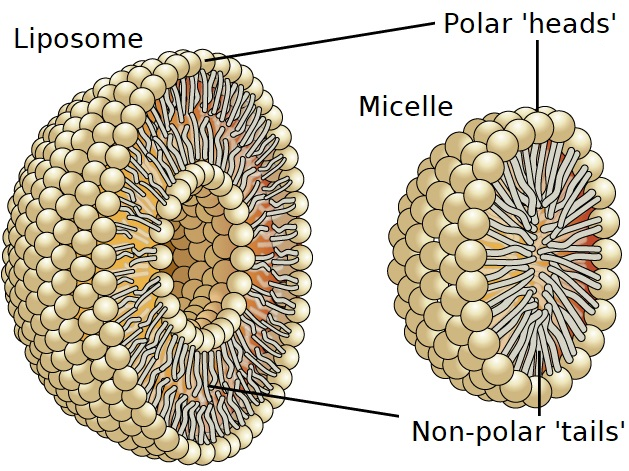
\includegraphics[width=0.55\textwidth,height=\textheight]{figures/ch3/OSC_Microbio_07_03_micelle_edit.png}

}

\caption{\label{fig-micelle}Liposomes and micelles are made up of a
lipid membrane, which acts as a substitute for the cell membrane
\emph{in vitro}. Adapted from \autocite{Micelle}.}

\end{figure}

Nanodiscs have a particularly high stability compared to other formats
as their disc-shaped lipid bilayer is encompassed by a membrane scaffold
protein (MSP) \autocite{Nath2007,Bayburt2010}. The stability of this
format means it is frequently used in the fabrication of biosensor
devices, which are often described as being particularly reliable and
long-lived \autocite{Goldsmith2011,Yang2018,Moon2020,Cheema2021}.
Another advantage of nanodiscs is that the membrane scaffold protein can
be attached to biosensor surfaces at specific affinity tags, for
example, the MSP hexahistidine tag (`his-tag') \autocite{Bayburt2010}.
Unlike other artificial membranes, there is also little variation
between the size of individual nanodiscs \autocite{Nath2007}. Depending
on the type of MSP used, a nanodisc measures between 10-20 nm across and
can hold either a single or several odorant receptors
\autocite{Nath2007,Bayburt2010}. Figure~\ref{fig-msp-iOR-nanodisc} shows
the structure of a nanodisc with contained odorant receptors.

\begin{figure}

{\centering 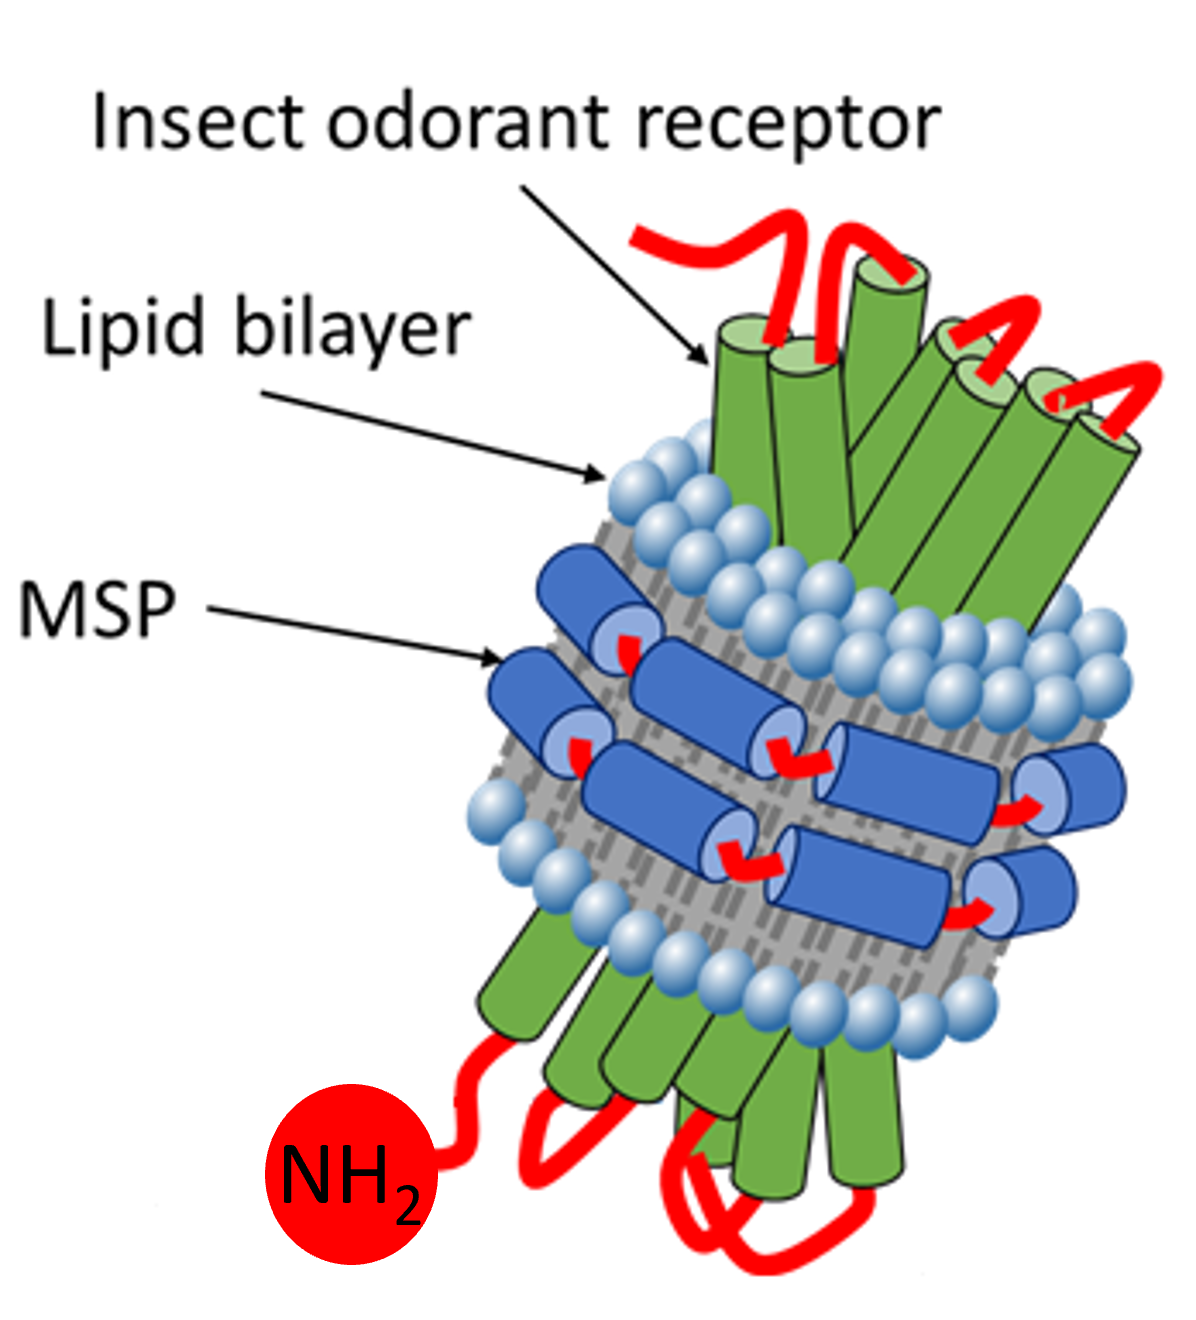
\includegraphics[width=0.4\textwidth,height=\textheight]{figures/ch3/iOR_nanodisc.png}

}

\caption{\label{fig-msp-iOR-nanodisc}A nanodisc containing an insect
odorant receptor transmembrane protein. MSP \(-\) membrane scaffold
protein. Reproduced with permission from \autocite{Murugathas2019a}.}

\end{figure}

\hypertarget{odorant-receptor-carbon-nanotube-and-graphene-biosensors}{%
\section{Odorant Receptor Carbon Nanotube and Graphene
Biosensors}\label{odorant-receptor-carbon-nanotube-and-graphene-biosensors}}

\hypertarget{sec-sensor-types}{%
\subsection{Sensor Functionalisation}\label{sec-sensor-types}}

Odorant receptors are highly sensitive and selective, making them
suitable as the biological sensing elements in a bioelectronic nose
\autocite{Dung2018}. There are multiple advantages to the use of odorant
receptors over a whole olfactory cell, including their smaller size and
relatively high stability \autocite{Dung2018}. Odorant receptors can be
expressed and isolated for sensor use using heterologous cell systems,
where a host cell replicates a protein from transfected RNA or DNA
material. The most commonly used expression cells are human embryonic
kidney (HEK) cells, \emph{E. Coli} bacteria and \emph{S. cerevisiae}
(baker's yeast) \autocite{Dung2018}.

For a bioelectronic nose to operate, sufficient coupling must exist
between the bioreceptor element and the sensor transducer. Odorant
receptors can be directly attached by physical adsorption; however, this
approach is difficult to control, and can result in weak coupling
between the odorant receptors and the transducer \autocite{Dung2018}.
Alternatively, a bifunctional linker element may mediate the attachment
between functional groups of the bioreceptor and the transducer in a
biochemical process referred to as functionalisation
\autocite{Star2003a}. The linker chemical interacts with the carbon-ring
surface either through stronger covalent bonding or weaker non-covalent
bonding. A more thorough comparison of covalent and non-covalent linker
functionalisation can be found in
\textbf{?@sec-noncovalent-functionalisation}.

\hypertarget{tbl-functionalisation-types}{}
\begin{longtable}[t]{>{\raggedright\arraybackslash}p{5.4cm}>{\raggedright\arraybackslash}p{1.45cm}>{\raggedright\arraybackslash}p{1.3cm}>{\raggedright\arraybackslash}p{1.45cm}>{\raggedright\arraybackslash}p{1.3cm}>{\raggedright\arraybackslash}p{1.3cm}}
\caption{\label{tbl-functionalisation-types}A comparison of the advantages and disadvantages of different approaches
for immobilising odorant receptors onto carbon nanotube or graphene
transducers. Simplicity = the amount of cost, time and effort involved
in functionalisation; Stability = the ability for the sensor to operate
over a long time and under a range of conditions; Specificity = the
ability to attach the receptor in a controlled and directional manner;
Strength = the strength of attachment between receptor and transducer;
Synergy = the ability for the receptor to attach without negatively
impacting transducer operation. }\tabularnewline

\toprule
Attachment Type & Simplicity & Strength & Specificity & Stability & Synergy\\
\midrule
Direct Adsorption & High & Low & Low & Low & Medium\\
Linker, non-covalently tethered & Medium & Medium & Medium & Medium & High\\
Linker, covalently tethered & Medium & High & High & High & Low\\
\bottomrule
\end{longtable}

\newpage
\KOMAoptions{paper=landscape,pagesize}

\hypertarget{tbl-or-biosensors}{}
\begin{longtable}[]{@{}llllllll@{}}
\caption{\label{tbl-or-biosensors}Summary of past fabrication methods
for odorant receptor-functionalised carbon nanotube and graphene
biosensors. GA = glutaraldehyde, DAN = 1,5-diaminonaphthalene, DMT-MM =
4-(4,6-dimethoxy-1,3,5-triazin-2-yl)-4 methylmorpholinium chloride, NTA
= nitrilotriacetic acid, PDL = poly-D-lysine, Ab = Antibody fragments,
CNTFET = carbon nanotube field-effect transistor, GFET = graphene
field-effect transistor, TX = transfer characteristics.}\tabularnewline
\toprule\noalign{}
Attachment & Attachment Method & References & Transducer & OR Type & OR
Format & Verification & LOD \\
\midrule\noalign{}
\endfirsthead
\toprule\noalign{}
Attachment & Attachment Method & References & Transducer & OR Type & OR
Format & Verification & LOD \\
\midrule\noalign{}
\endhead
\bottomrule\noalign{}
\endlastfoot
Direct & Vacuum-drying & Kim, 2009. \cite{Kim2009a} & CNTFET & Human &
Cell membrane & TEM & 100 fM \\
Non-covalent & GA-conjugated DAN & Park, 2012. \cite{Park2012} & GFET &
Human & Cell membrane & TX, SEM & 0.04 fM \\
& & Lee, 2012. \cite{Lee2012b} & CNTFET & Human & Cell membrane &
Fluorescence & 1 fM \\
& & Kwon, 2015. \cite{Kwon2015} & GFET & Human & Cell membrane & TEM &
0.1 fM \\
& & Goodwin, 2021. \cite{Goodwin2021} & GFET & Human & Cell membrane &
AFM, Raman & 0.5 pM \\
& PBASE & Murugathas, 2019. \cite{Murugathas2019a} & CNTFET & Insect &
Nanodiscs & TX, AFM & 1 fM \\
& & Murugathas, 2020. \cite{Murugathas2020} & GFET & Insect &
Nanovesicles, Nanodiscs & TX, AFM & 1 fM \\
& & Ahn, 2020. \cite{Ahn2020} & GFET & Human & Nanovesicles & TX, SEM &
100 fM \\
& & Yoo, 2022. \cite{Yoo2022} & CNTFET & Human & Micelles & TX, AFM & 1
fM \\
& DMT-MM & Yoon, 2009. \cite{Yoon2009} & CNTFET & Human & Cell membrane
& TX, SEM & 10 fM \\
Covalent & Diazonium salt/Ni-NTA & Goldsmith, 2011. \cite{Goldsmith2011}
& CNTFET & Mouse & Micelles, Nanodiscs & TX & \textasciitilde7 ppb \\
& & Son, 2017. \cite{Son2017} & CNTFET & Human & Micelles & TX, AFM & 10
fM \\
& PDL & Jin, 2012. \cite{Jin2012} & CNTFET & Human & Nanovesicles & SEM
& 1 fM \\
& & Park, 2012. \cite{Park2012a} & CNTFET & Dog & Nanovesicles & SEM & 1
fM \\
& & Lim, 2014. \cite{Lim2014} & CNTFET & Human & Nanovesicles & AFM & 10
fM \\
& & Lim, 2015. \cite{Lim2015} & CNTFET & Human & Nanovesicles & AFM & 1
fM \\
& & Son, 2015. \cite{Son2015} & CNTFET & Human & Nanovesicles & TX, SEM
& 10 ng/L \\
& & Ahn, 2015. \cite{Ahn2015} & CNTFET & Human & Nanovesicles & AFM & 1
fM \\
& Half-v5 mouse Ab & Lee, 2018. \cite{Lee2018} & CNTFET & Human &
Nanodiscs & TX, AFM, SEM & 1 fM \\
\end{longtable}

\newpage
\KOMAoptions{paper=portrait,pagesize}

\hypertarget{sec-biosensor-methods}{%
\subsection{Sensing Methods}\label{sec-biosensor-methods}}

In the nanovesicle or liposome-based odorant receptor biosensors shown
here, the presence of analyte triggers cell signalling which leads to
accumulation of ionic charge in the nanovesicle which the transducer
detects. The biosensors using other formats receive a signal from
binding of analyte to the receptor, which alters the distribution of
charge relative to the transducer \autocite{Dung2018}.

\hypertarget{aqueous-environment}{%
\subsubsection*{Aqueous Environment}\label{aqueous-environment}}
\addcontentsline{toc}{subsubsection}{Aqueous Environment}

\hypertarget{vapour-environment}{%
\subsubsection*{Vapour Environment}\label{vapour-environment}}
\addcontentsline{toc}{subsubsection}{Vapour Environment}

\begin{figure}

{\centering 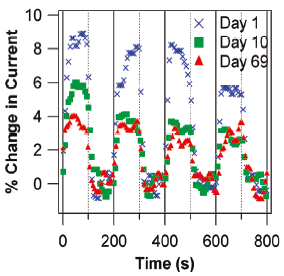
\includegraphics[width=0.4\textwidth,height=\textheight]{figures/ch3/eugenol.png}

}

\caption{\label{fig-eugenol-responses}Real-time responses to 2 ppm
eugenol vapour by an mOR174-9 nanodisc-functionalised single-CNT field
effect transistor. The response to eugenol on day 69 (red triangles)
indicates that the device retains the ability to respond to eugenol 10
weeks after functionalisation. Reproduced with permission from
\autocite{Goldsmith2011}.}

\end{figure}

Goldsmith \emph{et al.} have previously demonstrated it is possible to
specifically detect eugenol vapour using a single-CNT device
functionalised with mOR174-9 odorant receptors in either a surfactant
(digitonin) or nanodisc format. In the first study of this kind, the mOR
CNT FETs were exposed to nitrogen flow at 50\% relative humidity. The
resistance across a device gated at \(V_g\) = 0 V was measured while a
specific concentration of the positive ligand eugenol was added to the
constant flow for 100 s, then removed from the flow for 100 s. This
cycle was repeated five times. Figure~\ref{fig-eugenol-responses} shows
that significant real-time current increases of up to \(\sim\) 9\% were
observed during each cycle of exposure to eugenol. The device still
responded to eugenol cycles after 69 days of storage in 25\% (v/v)
ethanol at 4°C. This nicely-behaved and persistent activity may result
from the long-lived nanodisc format used \autocite{Goldsmith2011}. As
far as the author knows, there has been no investigation up until now
into whether this behaviour can be replicated for insect odorant
receptor devices. It is not clear that iORs can simply be substituted
for mORs for vapour sensing. The reasons for this distinction are made
in the subsequent section.

\hypertarget{insect-odorant-receptor-biosensors}{%
\section{Insect Odorant Receptor
Biosensors}\label{insect-odorant-receptor-biosensors}}

\hypertarget{in-vivo-structure-and-function-1}{%
\subsection{\texorpdfstring{\emph{In Vivo} Structure and
Function}{In Vivo Structure and Function}}\label{in-vivo-structure-and-function-1}}

Insect odorant (or olfactory) receptors (iORs) are a diverse range of
odorant-sensitive transmembrane proteins located in dendrite cells of
sensory hairs, known as sensilla, on the antennae and maxillary palps of
an insect \autocite{Clyne1999,Wicher2021}. Insects possess a specific
set of iORs tailored towards their ecological role (iORx, where the
``x'' denotes the OR variant), as well as a co-receptor known as
``ORCO'' (Odorant Receptor Co-Receptor). In the insect, a given iORx is
activated by volatile compounds, while the ORCO co-receptor is
insensitive to VOCs but couples with iORx to form a heteromeric complex,
which activates intracellular signalling via its ion channel activity.
\emph{In vivo}, the complex is required for VOC detection and operates
as a non-selective cation channel. This channel opens to allow ions to
travel across the cell membrane in response to iOR interaction with VOCs
\autocite{Smart2008,Wicher2008,Sato2008,Carraher2015,Butterwick2018,Wicher2021,Cheema2021}.

iORs were initially thought to be similar in structure to vertebrate
odorant receptors, but is now known that iORs have a completely
different topology and mechanism to GPCRs, despite also possessing
seven-transmembrane domains. Their configuration in the membrane is
inverted. Equivalently, the carboxyl group or `C terminus' of the iOR
sits outside the membrane of a cell, and the anime group or `N terminus'
of the iOR sits inside the cell membrane
\autocite{Glatz2011,Butterwick2018,Carraher2015}.

Each odorant receptor of the \emph{Drosophilia melanogaster} sensilla
will respond to a variety of odor compound. Odors which provoke a
particularly strong response from a specific odorant receptor are
referred to in the literature as `positive ligands' for that receptor
\autocite{Murugathas2019a,Murugathas2020}. The strength of response by a
specific OR depends on the compound being detected; furthermore, there
may be no response to a compound, or one compound may inhibit the
response of the receptor to other compounds. Odor compounds which
provoke no response from a particular receptor are referred to as
`negative ligands' for that receptor
\autocite{Murugathas2019a,Murugathas2020}. A comprehensive database that
details the various \emph{Drosophilia melanogaster} odorant receptors
and their response profile to a range of volatile compounds can be
consulted online \autocite{Munch2016}.

\hypertarget{aqueous-sensing}{%
\subsection{Aqueous Sensing}\label{aqueous-sensing}}

As in the case of vertebrate ORs, recent studies have shown that iORs
each interact with a specific VOC or a specific range of VOCs and can
also be used in bioelectronic nose applications. However, the sensing
mechanisms underlying their use \emph{in vitro} are not currently
well-understood \autocite{Murugathas2019a,Murugathas2020,Khadka2019}.
From further development and examination of iOR-based biosensors, new
insights into the mechanisms at play may emerge. Previously, the
literature has primarily focused on the operation of iOR-FET biosensors
in an aqueous environment. Here, carbon nanotube or graphene FETs have
been non-covalently functionalised with insect odorant receptors in
either a nanodisc or liposome format. The high surface-to-volume ratio
of carbon nanotubes and graphene allow for the odorant receptors to be
densely immobilised across the channel surface. The functionalised
channel is placed in a liquid-gated environment contained in
polydimethylsiloxane (PDMS) and gated with a Ag-AgCl reference electrode
(see \textbf{?@sec-gating}). Phosphate buffered saline (PBS) is used as
the liquid gate electrolyte \autocite{Murugathas2019a,Murugathas2020}. A
small amount of DMSO is also added to the electrolyte, a dipolar solvent
which is widely used to solubilise poorly soluble analytes in a
biological setting \autocite{Galvao2014}.

\begin{figure}

\begin{minipage}[t]{0.03\linewidth}

{\centering 

\raisebox{-\height}{


\includegraphics{figures/(a).png}

}

}

\end{minipage}%
%
\begin{minipage}[t]{0.01\linewidth}

{\centering 

~

}

\end{minipage}%
%
\begin{minipage}[t]{0.45\linewidth}

{\centering 

\raisebox{-\height}{

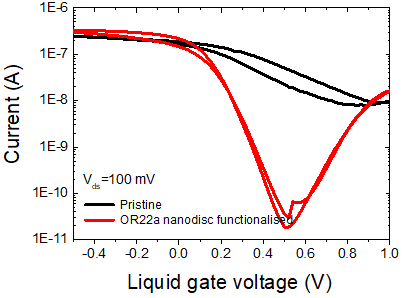
\includegraphics{figures/ch3/OR22a_ND_CNTFET.png}

}

}

\end{minipage}%
%
\begin{minipage}[t]{0.01\linewidth}

{\centering 

~

}

\end{minipage}%
%
\begin{minipage}[t]{0.03\linewidth}

{\centering 

\raisebox{-\height}{


\includegraphics{figures/(b).png}

}

}

\end{minipage}%
%
\begin{minipage}[t]{0.01\linewidth}

{\centering 

~

}

\end{minipage}%
%
\begin{minipage}[t]{0.45\linewidth}

{\centering 

\raisebox{-\height}{

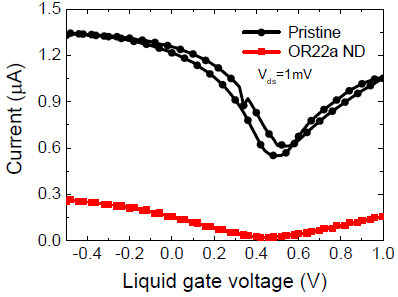
\includegraphics{figures/ch3/OR22a_ND_GFET.png}

}

}

\end{minipage}%
%
\begin{minipage}[t]{0.01\linewidth}

{\centering 

~

}

\end{minipage}%
\newline
\begin{minipage}[t]{0.03\linewidth}

{\centering 

\raisebox{-\height}{


\includegraphics{figures/(c).png}

}

}

\end{minipage}%
%
\begin{minipage}[t]{0.01\linewidth}

{\centering 

~

}

\end{minipage}%
%
\begin{minipage}[t]{0.45\linewidth}

{\centering 

\raisebox{-\height}{

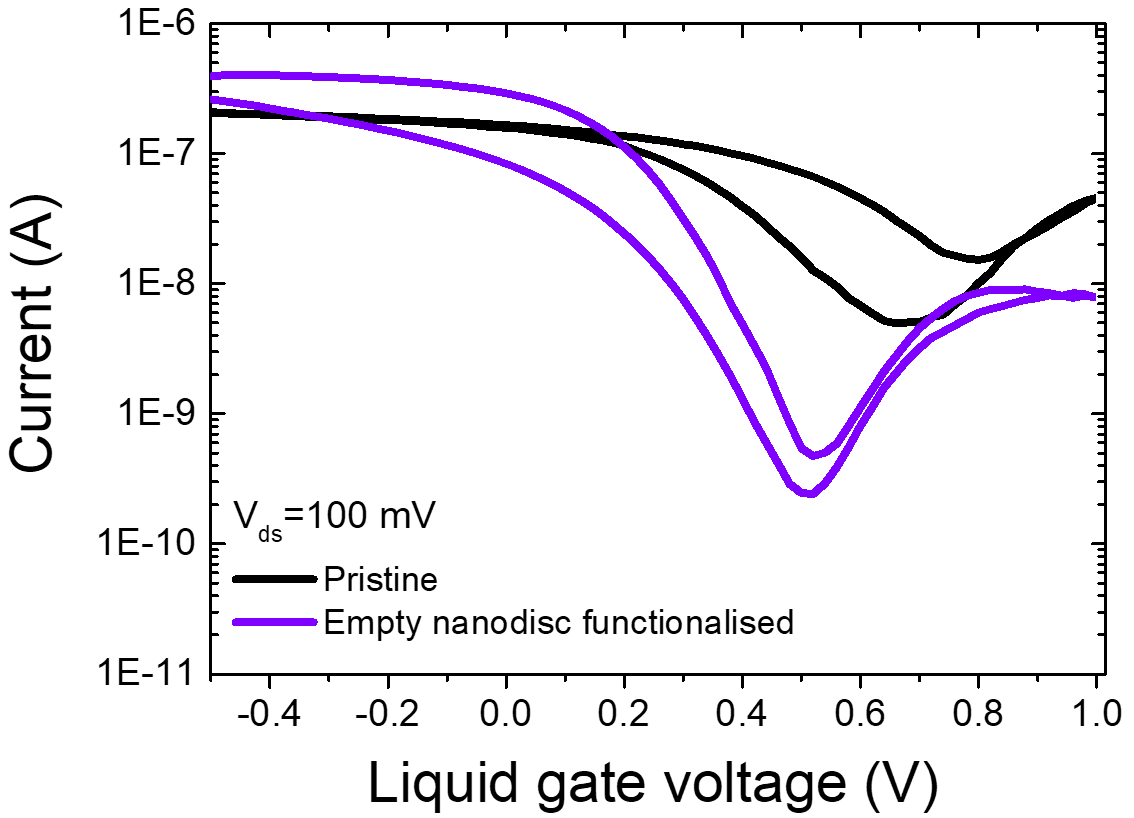
\includegraphics{figures/ch3/Empty_ND_CNTFET.png}

}

}

\end{minipage}%
%
\begin{minipage}[t]{0.01\linewidth}

{\centering 

~

}

\end{minipage}%
%
\begin{minipage}[t]{0.03\linewidth}

{\centering 

\raisebox{-\height}{

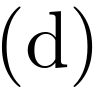
\includegraphics{figures/(d).png}

}

}

\end{minipage}%
%
\begin{minipage}[t]{0.01\linewidth}

{\centering 

~

}

\end{minipage}%
%
\begin{minipage}[t]{0.45\linewidth}

{\centering 

\raisebox{-\height}{

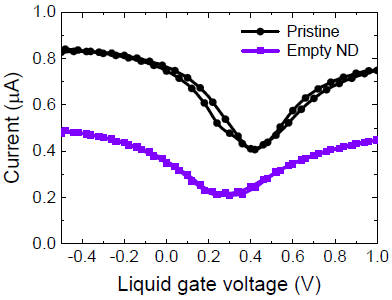
\includegraphics{figures/ch3/Empty_ND_GFET.png}

}

}

\end{minipage}%
%
\begin{minipage}[t]{0.01\linewidth}

{\centering 

~

}

\end{minipage}%

\caption{\label{fig-functionalisation-literature}Transfer characteristic
curves before and after functionalisation of (a) an OR22a
nanodisc-functionalised CNT network FET, (b) an OR22a
nanodisc-functionalised graphene FET, (c) an empty
nanodisc-functionalised CNT network FET and (d) an empty
nanodisc-functionalised graphene FET. Reproduced with permission from
\autocite{Murugathas2019a,Murugathas2020}.}

\end{figure}

Functionalisation of a FET device channel with iORs significantly alters
the transfer characteristics of that channel. Murugathas \emph{et al.}
found that successful functionalisation of a CNTFET device with iORs
would typically increase the device on-current, increase its on-off
ratio and cause a significant negative shift in threshold voltage, as
shown in Figure~\ref{fig-functionalisation-literature} (a)
\autocite{Murugathas2019a}. Meanwhile, successful functionalisation of a
graphene device with iORs would typically dramatically decrease the
device on-current and cause a negative shift in Dirac voltage, as seen
in Figure~\ref{fig-functionalisation-literature} (b)
\autocite{Murugathas2020}. These changes are not simply the result of
linker attachment to the channel surface \autocite{Murugathas2019a}. It
is thought that the negative shift of both threshold and Dirac voltages
are caused by the N-terminus amine groups on the odorant receptors or
amine groups on the nanodisc membrane scaffold proteins donating
electrons to the device channel, which has a similar effect to doping
the channel with impurities
\autocite{Bradley2004,Murugathas2019a,Murugathas2020}. Note that very
similar changes occur when functionalising with empty nanodiscs which
contain no odorant receptors, shown in
Figure~\ref{fig-functionalisation-literature} (c) and
Figure~\ref{fig-functionalisation-literature} (d). Unless the odorant
receptors attach preferentially to the network over nanodiscs, it
appears the gating effect is predominantly due to the large-scale
attachment of nanodisc membranes.

\begin{figure}

\begin{minipage}[t]{0.03\linewidth}

{\centering 

\raisebox{-\height}{


\includegraphics{figures/(a).png}

}

}

\end{minipage}%
%
\begin{minipage}[t]{0.01\linewidth}

{\centering 

~

}

\end{minipage}%
%
\begin{minipage}[t]{0.45\linewidth}

{\centering 

\raisebox{-\height}{

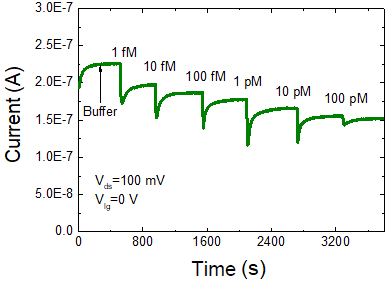
\includegraphics{figures/ch3/OR22a_realtime_normalised_CNTFET_1.png}

}

}

\end{minipage}%
%
\begin{minipage}[t]{0.01\linewidth}

{\centering 

~

}

\end{minipage}%
%
\begin{minipage}[t]{0.03\linewidth}

{\centering 

\raisebox{-\height}{


\includegraphics{figures/(b).png}

}

}

\end{minipage}%
%
\begin{minipage}[t]{0.01\linewidth}

{\centering 

~

}

\end{minipage}%
%
\begin{minipage}[t]{0.45\linewidth}

{\centering 

\raisebox{-\height}{

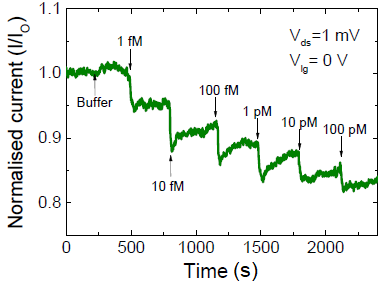
\includegraphics{figures/ch3/OR22a_realtime_normalised_GFET_1.png}

}

}

\end{minipage}%
%
\begin{minipage}[t]{0.01\linewidth}

{\centering 

~

}

\end{minipage}%
\newline
\begin{minipage}[t]{0.03\linewidth}

{\centering 

\raisebox{-\height}{


\includegraphics{figures/(c).png}

}

}

\end{minipage}%
%
\begin{minipage}[t]{0.01\linewidth}

{\centering 

~

}

\end{minipage}%
%
\begin{minipage}[t]{0.45\linewidth}

{\centering 

\raisebox{-\height}{

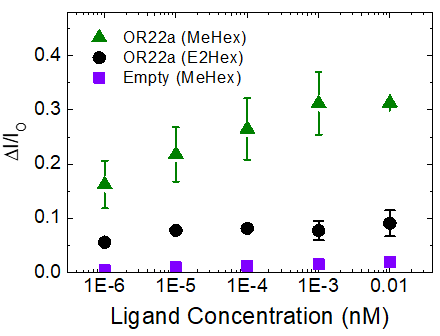
\includegraphics{figures/ch3/OR22a_realtime_normalised_CNTFET_2.png}

}

}

\end{minipage}%
%
\begin{minipage}[t]{0.01\linewidth}

{\centering 

~

}

\end{minipage}%
%
\begin{minipage}[t]{0.03\linewidth}

{\centering 

\raisebox{-\height}{

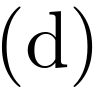
\includegraphics{figures/(d).png}

}

}

\end{minipage}%
%
\begin{minipage}[t]{0.01\linewidth}

{\centering 

~

}

\end{minipage}%
%
\begin{minipage}[t]{0.45\linewidth}

{\centering 

\raisebox{-\height}{

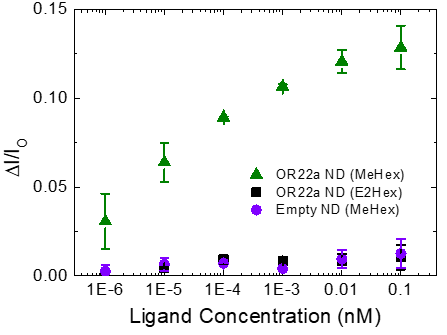
\includegraphics{figures/ch3/OR22a_realtime_normalised_GFET_2.png}

}

}

\end{minipage}%
%
\begin{minipage}[t]{0.01\linewidth}

{\centering 

~

}

\end{minipage}%

\caption{\label{fig-iOR-sensing-literature}Real-time responses to
concentrations of methyl hexanoate in \(1 \times\) phosphate buffer
saline (PBS) with 1\% v/v DMSO by (a) an OR22a nanodisc-functionalised
CNT network FET and (b) an OR22a nanodisc-functionalised graphene FET,
alongside the normalised signal response curves corresponding to (c) CNT
network FETs and (d) graphene FETs. The response curves show the
cumulative responses of OR22a-functionalised devices to both the
positive ligand methyl hexanoate (green) and negative ligand
\emph{trans}-2-hexan-1-al (black). They also show the cumulative
response of a empty nanodisc functionalised device to methyl hexanoate
(purple). Reproduced with permission from
\autocite{Murugathas2019a,Murugathas2020}.}

\end{figure}

Interactions between iORs attached to the channel, such as OR22a, and
positive ligands added to the electrolyte environment, such as methyl
hexanoate (MeHex), can alter the current flowing through the channel.
These current changes can be monitored over time and interpreted as
real-time sensor responses. Figure~\ref{fig-iOR-sensing-literature} (a)
and (b) show the respective responses of the OR22a-functionalised CNT
FET and graphene FET in Figure~\ref{fig-functionalisation-literature} to
methyl hexanoate in real-time. This result demonstrates that iOR-FETs
are sensitive down to the femtomolar scale in an aqueous environment.
Figure~\ref{fig-iOR-sensing-literature} (c) and (d) compare the average
methyl hexanoate responses of multiple devices to that of relevant
controls. It was verified that the OR22a-functionalised devices would
not respond to \emph{trans}-2-hexan-1-al, the negative ligand for OR22a;
it was also verified that empty nanodiscs would not respond
non-selectively to the positive ligand
\autocite{Murugathas2019a,Murugathas2020}.

\hypertarget{sensing-mechanisms}{%
\subsubsection*{Sensing Mechanisms}\label{sensing-mechanisms}}
\addcontentsline{toc}{subsubsection}{Sensing Mechanisms}

The reduction in the channel current of a functionalised FET upon
exposure to a positive ligand is notably different to the signal
transduction mechanism of iORs \emph{in vivo}, since ORCO does not
appear to be required for an iOR bioelectronic nose to function. It has
been proposed that the signal response results from the positive ligand
binding to the iOR protein, causing it to change shape. Cheema \emph{et
al.} used neutron reflectometry to demonstrate that OR22a nanodiscs
undergo a 1 nm height change after ethyl hexanoate exposure, likely
resulting from a structural change \autocite{Cheema2021}. This change
most likely affects the channel in one of two ways. The first involves
transfer of charge from the iOR to the channel, reducing I\(_{d}\) and
causing a negative threshold voltage (or Dirac point) shift. Another
could be a more indirect electrostatic gating effect, due to the
movement of charge within the Debye screening length of the channel. The
Debye length of \(1 \times\) PBS buffer is typically much shorter than
the height of a single nanodisc \autocite{Murugathas2019a}. However, if
structural changes in the iOR were primarily occurring at its base, it
is still possible that the electrostatic gating could be the primary
sensing mechanism.

\hypertarget{sec-non-specific-binding}{%
\section{Non-Specific Binding}\label{sec-non-specific-binding}}

Non-specific binding (NSB) refers to any attachment to the sensor
channel not related to the specific analyte of interest which could
interfere with sensing. Liquid-gated graphene and carbon nanotube
devices are highly sensitive to the approach of charge within the Debye
length of the device channel \autocite{Shkodra2021}. Non-specific
adsorption of the analyte or ambient contamination from numerous
elements used in fabricating the biosensor can lead to signal responses
not attributable to the mechanism of interest (see
\textbf{?@sec-CNT-sensing-mechanisms}), leading to false positives when
sensing \autocite{Chen2004,Star2003a,Shkodra2021}. Non-specific
adsorption can occur on the channel as well as the the source-drain and
gate electrodes \autocite{Chen2004}. A variety of measures can be taken
to prevent NSB from occurring. Once bioreceptors have been attached to
the channel, remaining exposed carbon nanotubes can be passivated with
chemical coatings such as Tween-20 \autocite{Chen2004}, PEG
\autocite{Star2003a}, and ethanolamine \autocite{Maehashi2007,Das2011}.
If measuring multiple channels in a multiplexed array, one channel can
be left uncoated to compare the sensing response in a process known as
`internal referencing' \autocite{Shkodra2021}.

Non-specific binding is particularly significant for
protein-functionalised devices. Proteins may be spontaneously adsorbed
onto carbon nanotube or graphene surfaces during functionalisation in a
manner which is not linker-mediated
\autocite{Bradley2004,Star2003a,Chen2004}. Such adsorption is known to
reduce the conductance of device channels containing semiconducting
carbon nanotubes, which may result from electron transfer between amino
acid residues and the nanotube network. The significance of this effect
is increased when electrodes are not sufficiently passivated or
encapsulated due to modulation of the Schottky barrier at the
metal-carbon nanotube interface \autocite{Chen2004}.

\cleardoublepage
\phantomsection
\addcontentsline{toc}{part}{Appendices}
\appendix

\hypertarget{sec-vapour-sensor-components}{%
\chapter{Vapour System Hardware}\label{sec-vapour-sensor-components}}

\hypertarget{tbl-vapour-sensor-components}{}
\begin{longtable}[t]{>{\raggedright\arraybackslash}p{5.5cm}>{\raggedright\arraybackslash}p{4.5cm}>{\raggedright\arraybackslash}p{3.75cm}}
\caption{\label{tbl-vapour-sensor-components}Major components used in construction of the vapour delivery system
described in this thesis. }\tabularnewline

\toprule
Description & Part No. & Manufacturer\\
\midrule
Mass flow controller, 20 sccm full scale & GE50A013201SBV020 & MKS Instruments\\
Mass flow controller, 200 sccm full scale & GE50A013202SBV020 & MKS Instruments\\
Mass flow controller, 500 sccm full scale & FC-2901V & Tylan\\
Analogue flowmeter, 240 sccm max. flow & 116261-30 & Dwyer\\
Micro diaphragm pump & P200-B3C5V-35000 & Xavitech\\
\addlinespace
Analogue flow controller, for micro diaphragm pump & X3000450 & Xavitech\\
10 mL Schott bottle & 218010802 & Duran\\
PTFE connection cap system & Z742273 & Duran\\
Baseline VOC-TRAQ flow cell, red & 043-951 & Mocon\\
Humidity and temperature sensor & T9602 & Telaire\\
\addlinespace
Enclosure, for humidity and temperature sensor & MC001189 & Multicomp Pro\\
\bottomrule
\end{longtable}

\hypertarget{sec-python}{%
\chapter{Python Code for Data Analysis}\label{sec-python}}

\hypertarget{code-repository}{%
\section{Code Repository}\label{code-repository}}

The code used for general analysis of field-effect transistor devices in
this thesis was written with Python 3.8.8. Contributors to the code used
include Erica Cassie, Erica Happe, Marissa Dierkes and Leo Browning. The
code is located on GitHub and the research group OneDrive, and is
available on request.

\hypertarget{sec-histogram-analysis}{%
\section{Atomic Force Microscope Histogram
Analysis}\label{sec-histogram-analysis}}

The purpose of this code is to analyse atomic force microscope (AFM)
images of carbon nanotube networks in .xyz format taken using an atomic
force microscope and processed in Gwyddion (see
\textbf{?@sec-afm-characterisation}). It was originally designed by
Erica Happe in Matlab, and adapted by Marissa Dierkes and myself for use
in Python. The code imports the .xyz data and sorts it into bins 0.15 nm
in size for processing. To perform skew-normal distribution fits, both
\emph{scipy.optimize.curve\_fit} and \emph{scipy.stats.skewnorm} modules
are used in this code.

\hypertarget{sec-raman-analysis}{%
\section{Raman Spectroscopy Analysis}\label{sec-raman-analysis}}

The purpose of this code is to analyse a series of Raman spectra taken
at different points on a single film (see
\textbf{?@sec-raman-characterisation}). Data is imported in a series of
tab-delimited text files, with the low wavenumber spectrum (100
cm\(^{-1} - 650\) cm\(^{-1}\)) and high wavenumber spectrum (1300
cm\(^{-1} - 1650\) cm\(^{-1}\)) imported in separate datafiles for each
scan location.

\hypertarget{sec-field-effect-transistor-analysis}{%
\section{Field-Effect Transistor
Analysis}\label{sec-field-effect-transistor-analysis}}

The purpose of this code is to analyse electrical measurements taken of
field-effect transistor (FET) devices. Electrical measurements were
either taken from the Keysight 4156C Semiconductor Parameter Analyser,
National Instruments NI-PXIe or Keysight B1500A Semiconductor Device
Analyser as discussed in \textbf{?@sec-electrical-characterisation}; the
code is able to analyse data in .csv format taken from all three
measurement setups. The main Python file in the code base consists of
three related but independent modules: the first analyses and plots
sensing data from the FET devices, the second analyses and plots
transfer characteristics from channels across a device, and the third
compares individual channel characteristics before and after a
modification or after each of several modifications. The code base also
features a separate config file and style sheet which govern the
behaviour of the main code. The code base was designed collaboratively
by myself and Erica Cassie over GitHub using the Sourcetree Git GUI.


\backmatter
\printbibliography


\end{document}
